\documentclass[twoside]{article}

%%%%%%%%%%%%%%%%%%%%%%%%%%%%%%%%%%%%%%%%%%%%%%%%%%%%%%%%%%%%%%%%%%%%%
% Packages

\usepackage[utf8]{inputenc}

% paper settings
\usepackage{geometry}

% macro helpers
\usepackage{xspace}
\usepackage{calc}
\usepackage{ifthen}
\usepackage{amsmath}
\usepackage{listofitems}

% tabular environments
\usepackage{array}
\usepackage{multirow}

% graphics and color
\usepackage{pict2e}
\usepackage[usenames]{color}
\usepackage{colortbl}

% special symbols
\usepackage{pifont}

\usepackage{afterpage}

%--------------------------------------------------------------------
% Document-wide settings

\input{DYI_config}
\geometry{portrait}
\geometry{inner=18mm,outer=10mm,top=10mm,bottom=10mm}

% Don't show page numbers
\pagestyle{empty}

% Default font: Avantgarde
%\usepackage{avant}
%\renewcommand{\familydefault}{pag}
\usepackage[sfdefault]{roboto}
\usepackage[T1]{fontenc}

% no paragraph indentation
\setlength{\parindent}{0pt}

% Color definitions
% - plain black
\definecolor{Black}{gray}{0}
% - disabled days in MonthlyPlanner (from prior/next month)
\definecolor{DayMPDisabled}{gray}{0.7}
% - table headers: month names in Year Calendar and MiniCal/MonthlyPlanner
\definecolor{HeadMainBg}{gray}{0.4}
% - table second header: day names in monthy calendars (incl MiniCal/MonthlyPlanner)
\definecolor{HeadSubBg}{gray}{0.8}
% - table column color for Sat, Sun (Weekend), uncomment & tune 2nd def for color
\definecolor{WeekendDay}{gray}{0.3}
% - writing guides - primary: (thin) rules/lines, dots, etc.
\definecolor{WriteBgMain}{gray}{0.6}
% - writing guides - secondary: grey (thick) bars, etc.
\definecolor{WriteBgSec}{gray}{0.9}
% - table header background in Monthly Planner
\definecolor{HeadMainBgMP}{gray}{0.8}

% Hacks
% - required by correct \rowcolor
\setlength{\tabcolsep}{0pt}

%--------------------------------------------------------------------
% Macros

% vertical strut
%	#1 (optional) = "lift", default 0pt
%	#2            = "(total)height"
\newcommand{\vstrut}[2][0pt]{\rule[#1]{0pt}{#2}}

% Internationalization
\input{DYI_i18n}

%%%%%%%%%%%%%%%%%%%%%%%%%%%%%%%%%%%%%%%%%%%%%%%%%%%%%%%%%%%%%%%%%%%%

\input{DYI_Month_Tables.tex}
\input{DYI_Monthly_Planner_Tables.tex}

%\newcounter{DIYYear}
%\setcounter{DIYYear}{\MyYear}

\usepackage[hyphens]{url}
\usepackage{rotating}
\usepackage{forloop}% http://ctan.org/pkg/forloop
\newcounter{loopcntr}
\newcommand{\rpt}[2][1]{%
  \forloop{loopcntr}{0}{\value{loopcntr}<#1}{#2}%
}
\usepackage{tikz}
\usepackage{latexsym}
\usepackage{multicol}
\usepackage{siunitx}

\newenvironment{checklist}{%
  \begin{list}{}{}% whatever you want the list to be
  \let\olditem\item
  \renewcommand\item{\olditem[$\Box$  $\Box$] }
}{%
  \end{list}
}

\begin{document}
\setcounter{secnumdepth}{0}
\include{fj_stuff}

%%%%%%%%%%%%%%%
% YEAR CALENDAR
%
% LAYOUT: 3 months per row, 4 rows (one page -- odd/right)
%					   <year>
%		---------------------------------
%		MONTH <space> MONTH <space> MONTH
%		MONTH <space> MONTH <space> MONTH
%		MONTH <space> MONTH <space> MONTH
%		MONTH <space> MONTH <space> MONTH
%		---------------------------------
%		---------------------------------
%		---------------------------------

% Settings-----------------------------------------------------------

% percentage (0.0 - 1.0) taken by the 3 months tables (3 months in a row) on the Year Calendar
% (the rest is equally split between 2 inter month-column spaces)
\newcommand\percentMonthColTWidthYC{0.95}

% calculate width of the month tabular* on the Year Calendar
\newlength{\MonthTblWidthYC}
\setlength{\MonthTblWidthYC}{( \textwidth * \real{\percentMonthColTWidthYC} ) / 3}

% calculate weekday column width inside the month tabular* on the Year Calendar
\newlength{\WkdayColWidthMonthTblYC}
\setlength{\WkdayColWidthMonthTblYC}{\MonthTblWidthYC / 7}

% Column Types for Months Tables on the Year Calendar
% Notes: - using 'tabular*' so use '@{\extracolsep\fill}')
%        - align to the 0.5em of right (supress the intercolumn space for better control)
%	 - color affects space (inserts struts in current font), put it after font change
% There are 4 types of columns
% - Column 1 (marked as weekend or weekday depending on week_starts_on_Monday value)
% This is output to DYI_i18n.tex
% - Column 2-5 (always weekday)
\newcolumntype{B}{>{\hfill\normalfont\footnotesize}p{\WkdayColWidthMonthTblYC}<{\hspace*{0.5em}}@{\extracolsep\fill}}
% - Column 6 (marked as weekend or weekday depending on week_starts_on_Monday value)
% This is output to DYI_i18n.tex
% - Column 7 (always weekend)
\newcolumntype{D}{>{\hfill\normalfont\footnotesize\color{WeekendDay}}p{\WkdayColWidthMonthTblYC}<{\hspace*{0.5em}}}

\newcommand{\MonthTblYC}[1]{%
	\begin{tabular*}{\MonthTblWidthYC}[t]{@{}A*{4}{B}CD@{}}
		\rowcolor{HeadSubBg}
		\WkdayTblRow{\bfseries\tiny} \\
		#1{\hfill}{\color{WeekendDay}\hfill}
	\end{tabular*}}

\newcommand{\MonthNameRowYC}[3]{%
	\rowcolor{HeadMainBg}
	\vstrut{1.1em}
	\color{white}#1 & \color{white}#2 & \color{white}#3}

% Start--------------------------------------------------------------

\hfill{\bfseries\Huge\MyYear}\par
\nointerlineskip\vspace{0.5em}
\rule{\textwidth}{1pt}

\nointerlineskip\vspace{0.5em}

\begin{tabular*}{\textwidth}{@{}>{\bfseries}c@{\extracolsep\fill}>{\bfseries}c@{\extracolsep\fill}>{\bfseries}c@{}}
	\MonthNameRowYC{\January}{\February}{\March}    \\
	\MonthTblYC{\MonthTblJan}  & \MonthTblYC{\MonthTblFeb}  & \MonthTblYC{\MonthTblMar} \\
	\MonthNameRowYC{\April}{\MayL}{\June}            \\
	\MonthTblYC{\MonthTblApr}  & \MonthTblYC{\MonthTblMay}  & \MonthTblYC{\MonthTblJun} \\
	\MonthNameRowYC{\July}{\August}{\September}     \\
	\MonthTblYC{\MonthTblJul}  & \MonthTblYC{\MonthTblAug}  & \MonthTblYC{\MonthTblSep} \\
	\MonthNameRowYC{\October}{\November}{\December} \\
	\MonthTblYC{\MonthTblOct}  & \MonthTblYC{\MonthTblNov}  & \MonthTblYC{\MonthTblDec}
\end{tabular*}

% fill the rest with lines, for notes
\vspace{2em}
{\color{WriteBgMain}
\rule{\textwidth}{1pt}\par
\rule{\textwidth}{1pt}\par
\rule{\textwidth}{1pt}\par
\rule{\textwidth}{1pt}\par
\rule{\textwidth}{1pt}\par
\rule{\textwidth}{1pt}\par
\rule{\textwidth}{1pt}\par
\rule{\textwidth}{1pt}\par}



\include{year_stuff}

%%%%%%%%%%%%%%%%%%%%%%%%%%%%%%%%%%%%%%%%%%%%%%%%%%%%%%%%%%%%%%%%%%%%%
%
%	MONTHLY PLANNER
%
%%%%%%%%%%%%%%%%%%%%%%%%%%%%%%%%%%%%%%%%%%%%%%%%%%%%%%%%%%%%%%%%%%%%%

% LAYOUT:       Odd Page:                   Even Page:
%		<Month>                   ||                <year>
%               --------------------------++----------------------
%               *Notes _| Mon | Tue | Wed || Thu | Fri | Sat | Sun
%		       _|     |     |     ||     |     |     |     <= 5 rows (6th will be crammed in 5th)
%               ..........................||......................
%               prior/next
%               month
%               mini cal.

% Settings-----------------------------------------------------------

% percentage (0.0 - 1.0) taken by the '*Notes' column out of the full quarter textwidth
\newcommand{\percentNoteColWidth}{0.95}
% reminder, easier to set explicitly, must add to 1.0
\newcommand{\percentNoteColWhite}{0.05}

% Column width in monthly planner: make room for rules
\newlength{\DayColWidthMP}
\setlength{\DayColWidthMP}{\textwidth / 4}

% Width of '*Notes' column
\newlength{\NoteColWidthMP}
\setlength{\NoteColWidthMP}{\DayColWidthMP * \real{\percentNoteColWidth}}
\newlength{\NoteColSkipMP}
\setlength{\NoteColSkipMP}{\DayColWidthMP * \real{\percentNoteColWhite}}

% Column Types for Days Columns in Monthly Planner
% - notes
\newcolumntype{N}{>{\centering}p{\NoteColWidthMP}@{\hspace\NoteColSkipMP}}
% - days, first/middle (Odd page: Mon, Tue; Even page: Thu, Fri, Sat)
\newcolumntype{M}{>{\centering}p{\DayColWidthMP}@{\extracolsep\fill}}
% - days, last (Odd page: Wed; Even page: Sun) \centering in combination with \\ doesn't work in last column, use \tabularnewline instead
\newcolumntype{O}{>{\centering\arraybackslash}p{\DayColWidthMP}@{}}

% Parameters for the month mini-calendars
% * Column types
\newlength{\WkdayColWidthMinicalMP}
\setlength{\WkdayColWidthMinicalMP}{\NoteColWidthMP / 7}
% There are 4 types of columns
% - Column 1 (marked as weekend or weekday depending on week_starts_on_Monday value)
% This is output to DYI_i18n.tex
% - Column 2-5 (always weekday)
\newcolumntype{F}{>{\hfill\bfseries\tiny}p{\WkdayColWidthMinicalMP}@{\extracolsep\fill}}
% - Column 6 (marked as weekend or weekday depending on week_starts_on_Monday value)
% This is output to DYI_i18n.tex
% - Column 7 (always weekend)(\vstrut is for the benefit of \color)
\newcolumntype{H}{>{\hfill\bfseries\tiny\vstrut{0pt}\color{WeekendDay}}p{\WkdayColWidthMinicalMP}}

% Tabular
\newcommand{\MonthMiniCalOnMonthlyPlanner}[2]{%
        \begin{tabular*}{\NoteColWidthMP}[t]{@{}E*{4}{F}GH@{}}
		\multicolumn{7}{>{\columncolor{HeadMainBg}}c}{\scriptsize\vstrut{1.1em}\bfseries\color{white}#1} \\
                \rowcolor{HeadSubBg}
                \WkdayTblRow{\hspace*{\fill}}\\
                #2{\hfill}{\color{WeekendDay}\hfill}
        \end{tabular*}}

% Notes column on odd page in Monthly Planner
% - hand tunned by trial and error, currently not posssible otherwise:
%   the heigh of the multirow is set up at the current evaluation based on current settings (font, etc)
% - so: artificially reserve (5 rows * 8 height) + 1 rows at current row heigh then build the minipage
% - last "8" reserved for building the previous/next months calendars
% Takes 4 params:
% - #1 previous month name
% - #2 previous month tabular layout
% - #3 next month name
% - #4 next month tabular layout
\newcounter{NotesColumnRows}%
\newcommand{\NoteColumn}[4]{%
	\multirow{41}{\NoteColWidthMP}{%
		\begin{minipage}{\NoteColWidthMP}%
			\makebox[0pt][l]{\smash[b]{\color{WriteBgSec}\rule[-24\baselineskip]{1em}{25\baselineskip}}}%
			{\color{WriteBgMain}\raggedright
				\setcounter{NotesColumnRows}{0}%
				\whiledo{\value{NotesColumnRows}<25}{%
					\rule{\NoteColWidthMP}{\arrayrulewidth}
					\stepcounter{NotesColumnRows}
				}%
			}%
		\end{minipage}%
		\break
		% previous month mini calendar
		\begin{minipage}{\NoteColWidthMP}%
			\renewcommand{\arraystretch}{0.8}
			\MonthMiniCalOnMonthlyPlanner{#1}{#2}
		\end{minipage}%
		\break
		% next month mini calendar
		\begin{minipage}{\NoteColWidthMP}%
			\renewcommand{\arraystretch}{0.8}
			\MonthMiniCalOnMonthlyPlanner{#3}{#4}
		\end{minipage}%
		\break \vspace{4.6pt} % push it to the top
	}%
}

% Cell format on Monthly Planner, pure play :)
% - template: #1 - color for day number and left rule, #2 - date number, #3 - event text to show on date
\newcommand{\CellFormatMPTemplate}[3]{%
	% gray bar at the top, ~ half row height
	\makebox[0pt][l]{\smash[b]{\color{WriteBgSec}\rule[0.4\baselineskip]{\DayColWidthMP}{0.5\baselineskip}}}%
	% thin rule to the left almost full heigh 
	{\color{#1}\rule[-6\baselineskip]{\arrayrulewidth}{6\baselineskip}}%
	% date numbers and event text
	\hspace{1ex}\parbox[t]{\DayColWidthMP-1.5ex}{\color{#1}\makebox[1.7ex][r]{#2}\\\scriptsize#3}%
	% white last row, makes the left sided line open/incomplete (does not join the one below)
	\vstrut{1em}}
% this one for cramming 2 days in one table cell, for months spanning 6 rows
% - template: #1 - color for day number and left rule, #2 - first date number, #3 second date number,
% -  #4 first date event text, #5 second date event text
\newcommand{\CellFormatMPTemplateTwo}[5]{%
	% gray bar at the top, ~ half row height
	\makebox[0pt][l]{\smash[b]{\color{WriteBgSec}\rule[0.4\baselineskip]{\DayColWidthMP}{0.5\baselineskip}}}%
	% thin rule to the left almost full heigh 
	{\color{#1}\rule[-2.5\baselineskip]{\arrayrulewidth}{2.5\baselineskip}}%
	% date numbers and event text
	\hspace{1ex}\parbox[t]{\DayColWidthMP-1.5ex}{\color{#1}\makebox[1.7ex][r]{#2}\\\scriptsize#4}%
	\break%
	% white last row, makes the left sided line open/incomplete (does not join the one below)
	\vstrut{1em}%
	% repeat
	\makebox[0pt][l]{\smash[b]{\color{WriteBgSec}\rule[0.4\baselineskip]{\DayColWidthMP}{0.5\baselineskip}}}%
	{\color{#1}\rule[-2.5\baselineskip]{\arrayrulewidth}{2.5\baselineskip}}%
	\hspace{1ex}\parbox[t]{\DayColWidthMP-1.5ex}{\color{#1}\makebox[1.7ex][r]{#3}\\\scriptsize#5}%
	\break%
	\vstrut{1em}}

% for days in current month
% the optional argument is for months spanning 6 rows
\newcommand{\CellFormatMP}[4][]{%
	\ifthenelse{\equal{#1}{}}%
		{\CellFormatMPTemplate{Black}{#2}{#3}}%
		{\CellFormatMPTemplateTwo{Black}{#2}{#1}{#3}{#4}}}

% for days in previous/next month
\newcommand{\CellFormatMPDisabled}[2]{%
	\CellFormatMPTemplate{DayMPDisabled}{#1}{#2}}

% WARNING: The \vstrut in the heading for \MPLeftPage and \MPRightPage ensure enough space
%          (and proper alignmeng of the following table) when accented characters are used

% Monthly Planner Left Page
% takes 6 parameters:
% - #1   full name of current month
% - #2-5 are passed as #1-4 to \NoteColumn (see def)
% - #6   tabular layout for current month: \MP<Mon>Left
\newcommand{\MPLeftPage}[6]{%
	{\bfseries\Huge #1\vstrut[-0.5em]{1.4em}}\par
	\nointerlineskip
	\begin{tabular*}{\textwidth}{NMMO}
		\rowcolor{HeadMainBgMP}%
		% \makebox[1em] centers \ding{93} on the gray left vertical bar below, see \NoteColumn
		\bfseries\vstrut{1.1em}{\color{white}\makebox[1em]{\ding{93}}\ \ding{50}\hfill} & \bfseries\vstrut{1.1em}\color{white}\DayA & \bfseries\vstrut{1.1em}\color{white}\DayB & \bfseries\vstrut{1.1em}\color{white}\DayC \\
		% insert a dummy row: white, (cant use vspacing on previous \tabularnewline because it will turn colored as previous row)
		\\[-0.8em]
		\NoteColumn{#2}{#3}{#4}{#5}
			#6{\CellFormatMP}{\CellFormatMPDisabled}
	\end{tabular*}
	
	\clearpage
}

% Monthly Planner Right Page (similar to Right Page)
% takes 1 parameters:
% - #1    tabular layout for current month: \MP<Mon>Right
\newcommand{\MPRightPage}[1]{%
	\hfill{\bfseries\Huge\MyYear\vstrut[-0.5em]{1.4em}}\par
	\nointerlineskip

	\begin{tabular*}{\textwidth}{MMMO}
		\rowcolor{HeadMainBgMP}
		\bfseries\vstrut{1.1em}\color{white}\DayD & \bfseries\vstrut{1.1em}\color{white}\DayE & \bfseries\vstrut{1.1em}\color{white}\DayF & \bfseries\vstrut{1.1em}\color{white}\DayG \\
		% insert a dummy row: white, (cant use vspacing on previous \tabularnewline because it will turn colored as previous row)
		\\[-0.8em]
		#1{\CellFormatMP}{\CellFormatMPDisabled}
	\end{tabular*}

	\clearpage
}

\newcommand{\MyQuarter}{Q1}
\input{quarter_stuff}
% Start--------------------------------------------------------------

\MPLeftPage{\January}{\December}{\MonthTblDecPrev}{\February}{\MonthTblFeb}{\MPJanLeft}
\MPRightPage{\MPJanRight}

\MPLeftPage{\February}{\January}{\MonthTblJan}{\March}{\MonthTblMar}{\MPFebLeft}
\MPRightPage{\MPFebRight}

\MPLeftPage{\March}{\February}{\MonthTblFeb}{\April}{\MonthTblApr}{\MPMarLeft}
\MPRightPage{\MPMarRight}

\renewcommand{\MyQuarter}{Q2}
\input{quarter_stuff}

\MPLeftPage{\April}{\March}{\MonthTblMar}{\MayL}{\MonthTblMay}{\MPAprLeft}
\MPRightPage{\MPAprRight}

\MPLeftPage{\MayL}{\April}{\MonthTblApr}{\June}{\MonthTblJun}{\MPMayLeft}
\MPRightPage{\MPMayRight}

\MPLeftPage{\June}{\MayL}{\MonthTblMay}{\July}{\MonthTblJul}{\MPJunLeft}
\MPRightPage{\MPJunRight}

\renewcommand{\MyQuarter}{Q3}
\input{quarter_stuff}

\MPLeftPage{\July}{\June}{\MonthTblJun}{\August}{\MonthTblAug}{\MPJulLeft}
\MPRightPage{\MPJulRight}

\MPLeftPage{\August}{\July}{\MonthTblJul}{\September}{\MonthTblSep}{\MPAugLeft}
\MPRightPage{\MPAugRight}

\MPLeftPage{\September}{\August}{\MonthTblAug}{\October}{\MonthTblOct}{\MPSepLeft}
\MPRightPage{\MPSepRight}

\renewcommand{\MyQuarter}{Q4}
\input{quarter_stuff}

\MPLeftPage{\October}{\September}{\MonthTblSep}{\November}{\MonthTblNov}{\MPOctLeft}
\MPRightPage{\MPOctRight}

\MPLeftPage{\November}{\October}{\MonthTblOct}{\December}{\MonthTblDec}{\MPNovLeft}
\MPRightPage{\MPNovRight}

\MPLeftPage{\December}{\November}{\MonthTblNov}{\January}{\MonthTblJanNext}{\MPDecLeft}
\MPRightPage{\MPDecRight}



\include{DYI_Weekly_Planner}

\pgfmathsetmacro{\gridWidthCm}{\textwidth/1cm}
\newdimen\tikzspacer
\tikzspacer=18pt

\rpt[10]{
\section{dots}
\newdimen\spaceleft
\spaceleft=\dimexpr\textheight-\pagetotal-\tikzspacer\relax
\pgfmathsetmacro{\gridHeightCm}{\spaceleft/1cm}
% Needed to subtract an extra 14pt to prevent the page content from jumping
% to the next page in some cases.
  \begin{tikzpicture}
    \foreach \x in {0,0.5,...,\gridWidthCm}
    \foreach \y in {0,0.5,...,\gridHeightCm}
    {
  \fill (\x cm,\y cm) circle (0.015cm);
    }       
  \end{tikzpicture}
  \pagebreak
}
\rpt[10]{
  \section{triangular}
  \newdimen\spaceleft
  \spaceleft=\dimexpr\textheight-\pagetotal-\tikzspacer\relax
  \pgfmathsetmacro{\gridHeightCm}{\spaceleft/1cm}
  \begin{tikzpicture}
    \foreach \x [count=\xi] in {0,0.5,...,\gridWidthCm}
    \foreach \y [count=\yi] in {0,1,...,\gridHeightCm}
    {
  \fill (\x cm,\y cm) circle (0.015cm);
    }       
    \foreach \x [count=\xi] in {0.25,0.75,...,\gridWidthCm}
    \foreach \y [count=\yi] in {0.5,1.5,...,\gridHeightCm}
    {
  \fill (\x cm,\y cm) circle (0.015cm);
    }       
  \end{tikzpicture}
  \pagebreak
}
\rpt[6]{
 \section{graph}
  \newdimen\spaceleft
  \spaceleft=\dimexpr\textheight-\pagetotal-\tikzspacer\relax
  \pgfmathsetlengthmacro{\graphWidth}{\textwidth - mod(\textwidth,0.5cm)}
  \pgfmathsetlengthmacro{\graphHeight}{\spaceleft - mod(\spaceleft,0.5cm)}
  % Have to use mod here to get an even number of grid cells
  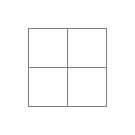
\begin{tikzpicture}
\draw [very thin, gray, step=0.5cm] (0,0) grid (\graphWidth,\graphHeight);
  \end{tikzpicture}
\pagebreak
}
\rpt[10]{
 \section{blank}
\pagebreak
}


\include{wireframe}
% We don't want any outside margins for the color pages
\newgeometry{inner=18mm,outer=0mm,top=0mm,bottom=0mm}

\includegraphics[width=\textwidth,height=\textheight]{./artwork/space}
\cleardoublepage
\includegraphics[width=\textwidth,height=\textheight]{./artwork/data_center}
\cleardoublepage
\includegraphics[width=\textwidth,height=\textheight]{./artwork/zengarden}
\cleardoublepage
\includegraphics[width=\textwidth,height=\textheight]{./artwork/london}
\cleardoublepage

\restoregeometry

\include{constants}
\include{ascii}
\include{numbers}
\end{document}
